\documentclass{standalone}
\usepackage{tikz}
\usetikzlibrary{patterns, positioning}


\begin{document}
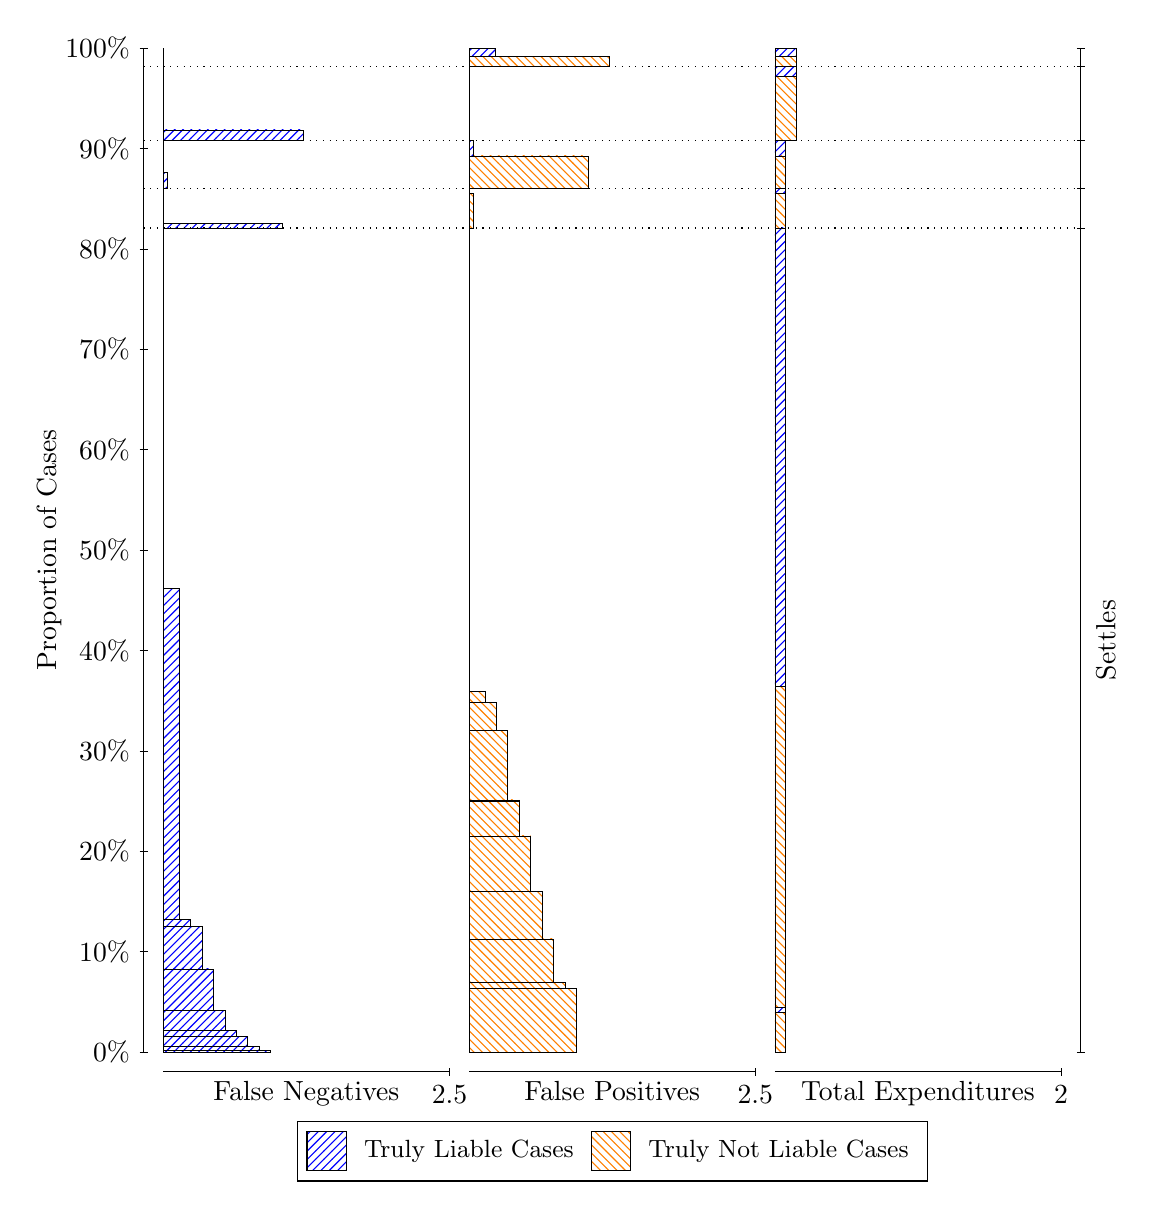
\begin{tikzpicture}
\draw[black, very thin] (1.5,1.75) -- (1.5,14.5);
\node[rotate=90, text=black, anchor=center] at (0.3, 8.125) {Proportion of Cases};
\draw[black, very thin] (1.45,1.75) -- (1.55,1.75);
\node[text=black, anchor=east] at (1.45, 1.75) {0\%};
\draw[black, very thin] (1.45,3.025) -- (1.55,3.025);
\node[text=black, anchor=east] at (1.45, 3.025) {10\%};
\draw[black, very thin] (1.45,4.3) -- (1.55,4.3);
\node[text=black, anchor=east] at (1.45, 4.3) {20\%};
\draw[black, very thin] (1.45,5.575) -- (1.55,5.575);
\node[text=black, anchor=east] at (1.45, 5.575) {30\%};
\draw[black, very thin] (1.45,6.85) -- (1.55,6.85);
\node[text=black, anchor=east] at (1.45, 6.85) {40\%};
\draw[black, very thin] (1.45,8.125) -- (1.55,8.125);
\node[text=black, anchor=east] at (1.45, 8.125) {50\%};
\draw[black, very thin] (1.45,9.4) -- (1.55,9.4);
\node[text=black, anchor=east] at (1.45, 9.4) {60\%};
\draw[black, very thin] (1.45,10.675) -- (1.55,10.675);
\node[text=black, anchor=east] at (1.45, 10.675) {70\%};
\draw[black, very thin] (1.45,11.95) -- (1.55,11.95);
\node[text=black, anchor=east] at (1.45, 11.95) {80\%};
\draw[black, very thin] (1.45,13.225) -- (1.55,13.225);
\node[text=black, anchor=east] at (1.45, 13.225) {90\%};
\draw[black, very thin] (1.45,14.5) -- (1.55,14.5);
\node[text=black, anchor=east] at (1.45, 14.5) {100\%};

\draw[black, very thin] (13.4,1.75) -- (13.4,14.5);
\draw[black, very thin] (13.35,1.75) -- (13.45,1.75);
\node[anchor=west] at (13.35, 1.75) {};
\draw[black, very thin] (13.35,12.215) -- (13.45,12.215);
\node[anchor=west] at (13.35, 12.215) {};
\draw[black, very thin] (13.35,12.714) -- (13.45,12.714);
\node[anchor=west] at (13.35, 12.714) {};
\draw[black, very thin] (13.35,13.331) -- (13.45,13.331);
\node[anchor=west] at (13.35, 13.331) {};
\draw[black, very thin] (13.35,14.271) -- (13.45,14.271);
\node[anchor=west] at (13.35, 14.271) {};
\draw[black, very thin] (13.35,14.5) -- (13.45,14.5);
\node[anchor=west] at (13.35, 14.5) {};

\draw[black, very thin, pattern color=blue, pattern=north east lines] (1.75,1.75) rectangle (3.1125,1.7679);
\draw[black, very thin, pattern color=blue, pattern=north east lines] (1.75,1.7679) rectangle (2.9672,1.8162);
\draw[black, very thin, pattern color=blue, pattern=north east lines] (1.75,1.8162) rectangle (2.8218,1.9511);
\draw[black, very thin, pattern color=blue, pattern=north east lines] (1.75,1.9511) rectangle (2.6765,2.0217);
\draw[black, very thin, pattern color=blue, pattern=north east lines] (1.75,2.0217) rectangle (2.5312,2.2787);
\draw[black, very thin, pattern color=blue, pattern=north east lines] (1.75,2.2787) rectangle (2.3858,2.8061);
\draw[black, very thin, pattern color=blue, pattern=north east lines] (1.75,2.8061) rectangle (2.2405,3.3484);
\draw[black, very thin, pattern color=blue, pattern=north east lines] (1.75,3.3484) rectangle (2.0952,3.4299);
\draw[black, very thin, pattern color=blue, pattern=north east lines] (1.75,3.4299) rectangle (1.9498,7.6346);
\draw[black, very thin, pattern color=orange, pattern=north west lines] (1.75,7.6346) rectangle (1.75,12.215);
\draw[black, very thin, pattern color=blue, pattern=north east lines] (1.75,12.215) rectangle (3.2578,12.271);
\draw[black, very thin, pattern color=orange, pattern=north west lines] (1.75,12.271) rectangle (1.75,12.714);
\draw[black, very thin, pattern color=blue, pattern=north east lines] (1.75,12.714) rectangle (1.8045,12.916);
\draw[black, very thin, pattern color=orange, pattern=north west lines] (1.75,12.916) rectangle (1.75,13.331);
\draw[black, very thin, pattern color=blue, pattern=north east lines] (1.75,13.331) rectangle (3.5303,13.459);
\draw[black, very thin, pattern color=orange, pattern=north west lines] (1.75,13.459) rectangle (1.75,14.271);
\draw[black, very thin, pattern color=orange, pattern=north west lines] (1.75,14.271) rectangle (1.75,14.396);
\draw[black, very thin, pattern color=blue, pattern=north east lines] (1.75,14.396) rectangle (1.75,14.5);
\draw[black, very thin, pattern color=orange, pattern=north west lines] (5.6333,1.75) rectangle (6.9958,2.5593);
\draw[black, very thin, pattern color=orange, pattern=north west lines] (5.6333,2.5593) rectangle (6.8505,2.6384);
\draw[black, very thin, pattern color=orange, pattern=north west lines] (5.6333,2.6384) rectangle (6.7052,3.1865);
\draw[black, very thin, pattern color=orange, pattern=north west lines] (5.6333,3.1865) rectangle (6.5598,3.7925);
\draw[black, very thin, pattern color=orange, pattern=north west lines] (5.6333,3.7925) rectangle (6.4145,4.4931);
\draw[black, very thin, pattern color=orange, pattern=north west lines] (5.6333,4.4931) rectangle (6.2692,4.9317);
\draw[black, very thin, pattern color=orange, pattern=north west lines] (5.6333,4.9317) rectangle (6.2692,4.9504);
\draw[black, very thin, pattern color=orange, pattern=north west lines] (5.6333,4.9504) rectangle (6.1238,5.8313);
\draw[black, very thin, pattern color=orange, pattern=north west lines] (5.6333,5.8313) rectangle (5.9785,6.185);
\draw[black, very thin, pattern color=orange, pattern=north west lines] (5.6333,6.185) rectangle (5.8332,6.3308);
\draw[black, very thin, pattern color=blue, pattern=north east lines] (5.6333,6.3308) rectangle (5.6333,12.215);
\draw[black, very thin, pattern color=orange, pattern=north west lines] (5.6333,12.215) rectangle (5.6878,12.658);
\draw[black, very thin, pattern color=blue, pattern=north east lines] (5.6333,12.658) rectangle (5.6333,12.714);
\draw[black, very thin, pattern color=orange, pattern=north west lines] (5.6333,12.714) rectangle (7.1412,13.13);
\draw[black, very thin, pattern color=blue, pattern=north east lines] (5.6333,13.13) rectangle (5.6878,13.331);
\draw[black, very thin, pattern color=orange, pattern=north west lines] (5.6333,13.331) rectangle (5.6333,14.143);
\draw[black, very thin, pattern color=blue, pattern=north east lines] (5.6333,14.143) rectangle (5.6333,14.271);
\draw[black, very thin, pattern color=orange, pattern=north west lines] (5.6333,14.271) rectangle (7.4137,14.396);
\draw[black, very thin, pattern color=blue, pattern=north east lines] (5.6333,14.396) rectangle (5.9603,14.5);
\draw[black, very thin, pattern color=orange, pattern=north west lines] (9.5167,1.75) rectangle (9.6529,2.2494);
\draw[black, very thin, pattern color=blue, pattern=north east lines] (9.5167,2.2494) rectangle (9.6529,2.3156);
\draw[black, very thin, pattern color=orange, pattern=north west lines] (9.5167,2.3156) rectangle (9.6529,6.397);
\draw[black, very thin, pattern color=blue, pattern=north east lines] (9.5167,6.397) rectangle (9.6529,12.215);
\draw[black, very thin, pattern color=orange, pattern=north west lines] (9.5167,12.215) rectangle (9.6529,12.658);
\draw[black, very thin, pattern color=blue, pattern=north east lines] (9.5167,12.658) rectangle (9.6529,12.714);
\draw[black, very thin, pattern color=orange, pattern=north west lines] (9.5167,12.714) rectangle (9.6529,13.13);
\draw[black, very thin, pattern color=blue, pattern=north east lines] (9.5167,13.13) rectangle (9.6529,13.331);
\draw[black, very thin, pattern color=orange, pattern=north west lines] (9.5167,13.331) rectangle (9.7892,14.143);
\draw[black, very thin, pattern color=blue, pattern=north east lines] (9.5167,14.143) rectangle (9.7892,14.271);
\draw[black, very thin, pattern color=orange, pattern=north west lines] (9.5167,14.271) rectangle (9.7892,14.396);
\draw[black, very thin, pattern color=blue, pattern=north east lines] (9.5167,14.396) rectangle (9.7892,14.5);
\draw[black, dotted] (1.5,12.215) -- (13.4,12.215);
\draw[black, dotted] (1.5,12.714) -- (13.4,12.714);
\draw[black, dotted] (1.5,13.331) -- (13.4,13.331);
\draw[black, dotted] (1.5,14.271) -- (13.4,14.271);
\draw[black, very thin] (1.75,1.5) -- (5.3833,1.5);
\node[text=black, anchor=north] at (3.5667, 1.5) {False Negatives};
\draw[black, very thin] (5.3833,1.45) -- (5.3833,1.55);
\node[text=black, anchor=north] at (5.3833, 1.45) {2.5};

\draw[black, very thin] (5.6333,1.5) -- (9.2667,1.5);
\node[text=black, anchor=north] at (7.45, 1.5) {False Positives};
\draw[black, very thin] (9.2667,1.45) -- (9.2667,1.55);
\node[text=black, anchor=north] at (9.2667, 1.45) {2.5};

\draw[black, very thin] (9.5167,1.5) -- (13.15,1.5);
\node[text=black, anchor=north] at (11.333, 1.5) {Total Expenditures};
\draw[black, very thin] (13.15,1.45) -- (13.15,1.55);
\node[text=black, anchor=north] at (13.15, 1.45) {2};

\node[text=black, centered, rotate=90] at (13.72, 6.9827) {Settles};





\draw (7.449999999999999,1.5) node[draw=none] (baseCoordinate) {};
\begin{scope}[align=center]
        \matrix[scale=0.5, draw=black, below=0.5cm of baseCoordinate, nodes={draw}, column sep=0.1cm]{
            \node[rectangle, draw, minimum width=0.5cm, minimum height=0.5cm, pattern color=blue, pattern=north east lines] {}; &
            \node[draw=none, font=\small, text=black] (B) {Truly Liable Cases}; &
            \node[rectangle, draw, minimum width=0.5cm, minimum height=0.5cm, pattern color=orange, pattern=north west lines] {}; &
            \node[draw=none, font=\small, text=black] (B) {Truly Not Liable Cases}; \\
            };
\end{scope}

\end{tikzpicture}
\end{document}